\documentclass{article}
\setlength{\oddsidemargin}{0.25 in}
\setlength{\evensidemargin}{-0.25 in}
\setlength{\topmargin}{-0.6 in}
\setlength{\textwidth}{6.5 in}
\setlength{\textheight}{8.5 in}
\setlength{\headsep}{0.75 in}
\setlength{\parindent}{0 in}
\setlength{\parskip}{0.1 in}

% ===== PACKAGES =====
\usepackage{amsmath,amssymb}
\usepackage{color}
\usepackage{float}
\usepackage{subfigure}
\usepackage{graphicx}
\usepackage{mdframed}
\usepackage{changepage}
\newmdenv[
  topline=false,
  bottomline=false,
  skipabove=\topsep,
  skipbelow=\topsep
]{siderules}
\renewcommand{\abstractname}{}

% ===== VARIABLES =====
\def \R{\mathbb{R}}
\def \Pr{\mathbb{P}}
\def \D{{\rm D}}
\def \N{{\rm N}}
\def \xx{{\boldsymbol{\rm x}}}
\def \y{{\rm y}}




% ===== HEADER BOX =====
\newcommand{\lecture}[2]{
\pagestyle{myheadings}
\thispagestyle{plain}
\newpage
\noindent
\begin{center}
\rule{\textwidth}{1.6pt}\vspace*{-\baselineskip}\vspace*{2pt} % Thick horizontal line
\rule{\textwidth}{0.4pt}\\[1\baselineskip] % Thin horizontal line
\vbox{\vspace{2mm}
\hbox to 6.28in { {\bf CS 760: Machine Learning} \hfill Spring 2022 }
\vspace{4mm}
\hbox to 6.28in { {\Large \hfill #1  \hfill} }
\vspace{4mm}
\hbox to 6.28in { {\scshape Authors:}  #2 \hfill }}
\vspace{-2mm}
\rule{\textwidth}{0.4pt}\vspace*{-\baselineskip}\vspace{3.2pt} % Thin horizontal line
\rule{\textwidth}{1.6pt}\\[\baselineskip] % Thick horizontal line
\end{center}
\vspace*{4mm}
}



% =============== DOCUMENT ===============
\begin{document}
\lecture{Models Predict Health and Biological Age from Incidental CT Data}{Zhiwei Song, Spencer Halberg-Spencer}

\begin{center}
{\Large {\sf \underline{\textbf{DO NOT POLLUTE!}} AVOID PRINTING, OR PRINT 2-SIDED MULTIPAGE.}}
\end{center}

\begin{abstract}
Machine Learning algorithms can be used to leverage large amounts of data to produce meaning models for prediction and classification. We have developed two machine learning models that can be used to classify patients risk for adverse heath effects using clinical and incidental computed tomography (CT) data. Our methods accurately predict individuals at risk for poor health outcomes including death. In addition to our classification models, we have developed a "biological age" metric that is computed using features from the CT and clinical data. We show that this metric is informative of poor health outcomes. 
\end{abstract}

\section{Introduction}
Clinical data has been used for decades to try and predict and treat medical conditions. Early attempts at developing meaning health metrics, such as BMI, create generalizable methods for accessing risks of individuals \cite{metropolitan1959new}. However, these metrics are inherently flawed because they do not account for the large amount of heterogeneity among individuals and include relatively few features \cite{freedmanValidityBMIIndicator2009}, \cite{nuttallBodyMassIndex2015}. Big data provides new opportunities for leveraging additional features that are a result of common medical examinations e.g. computed tomography (CT) \cite{hulsenBigDataPrecision2019}.  These incidental sources of data provide a rich collection of features that can be used to predict overall health in an individual. Machine learning algorithms leverage this data by incorporating multiple sources of information through a well understood framework that produce more generalizable predictions on health. In particular, many machine learning algorithms have been developed to incorporate clinical data to create methods for understanding wellbeing \cite{langarizadehApplyingNaiveBayesian2016}, \cite{goncalvesArtificialIntelligenceEarly2022}. We present our attempt to use incidental CT data with clinical data using two classification methods, naive Bayes and random forest.  Our models classify an individual into either a healthy group or at risk group. In addition to our classification models we present metric which we call "biological age" that incorporates  CT and clinical data to predict risk of adverse health effects. 

\section{Dataset}
The complete dataset consists of 9224 individuals and contains both clinical and statistics computed from Incidental computed tomography (CT) scans. We used the following features in preparing our dataset; BMI, sex, age at CT, the FRS 10-year risk score, the FRAX 10-year fracture probability, the FRAX 10-year hip fracture probability, bone mineral density, total fat, visceral fat, subcutaneous fat, the visceral-subcutaneous fat ratio, total body area, three muscle measures (HU, area and SMI), aortic calcification, liver fat, and indicators for tobacco usage, alcohol abuse, death, cardio vascular disease (CVD), heart failure, type 2 diabetes, fracture, Alzheimer's, and cancer. We generated the indicators without respect to the recorded  time of diagnosis since many of these conditions are results of longstanding health complications. For clinical conditions with multiple reported values, such as alcohol, we consider any reported value as an indicator of condition. From this dataset we built classifiers to predict the clinical outcomes of death, CVD, Alzheimer's, cancer, and diabetes. 

We prepared three datasets from the following data which we will denote as CT only, CT with clinical, and CT with clinical and condition indicators. The CT only data contains the statistics measured from the CT images and was used to predict the clinical conditions listed previously. The CT with clinical dataset includes all features except the indicators of death, CVD, Alzheimer's, cancer, and diabetes. Finally, the CT with clinical data and conditions contains all features including the clinical outcomes of CVD, Alzheimer's, cancer, and diabetes. Death was never used as a training feature because it is impractical to consider death as clinical features of living patients. When generating classifiers of the other clinical outcomes we removed the feature that we were trying to predict from the dataset to prevent training bias. Finally, for each of the three datasets, we removed individuals who did not contain all features or for which aberrant  values were reported because we did not want to impute clinical data that may bias our results. This resulted in a total of 8702 individuals in the CT only dataset, and 8113 individuals in the CT with clinical and CT with clinical and withdrawal dataset. 

\section{Approach}
This project consists of two main goals, to predict clinical outcomes from data, and to generate a biological age metric from the data. We will first present the methods used in prediction clinical features and compare the different machine learning algorithms.

\textbf{Naive Bayes Classifier:} We developed a framework for naive Bayes classification. For each feature the user can specify the distribution from a list of Gaussian, Bernoulli, exponential, Poison, Gamma, or Weibull distribution. Given a set of training pairs $\{(x_i, y_i)\}_{i=1}^N$, where $x_i are training features in \in \mathbb{R}^D$ and $y$ is an indicator of the clinical outcome that we are trying to predict, we select the value that maximizes the posterior probability under the assumption that each training feature is independent. We trained our model under the assumption that all non-indicator features in $x$ follow a normal distribution and indicator variables follow a Bernoulli distribution. We also tested where most non-indicator features were modeled as Gamma distributions and the remaining were modeled as exponential distributions. The Gamma distributions were selected because they better fit the skewed features in the data and increased the difference between the conditional distributions. 

\textbf{Stratified 5-fold Cross Validation:} To test the accuracy of the Naive Bayes classifier we used stratified 5-fold cross validation. We selected stratified 5-fold cross validation because the naive Bayes classifier is less susceptible to imbalance in classes then many other models and allows us to use the maximum amount of data for training. In stratified cross validation the data is partitioned into 5 folds where each fold contains the same proportion each class in the original dataset. The classifier is then trained on 4 of the 5 folds and tested on the remaining fold. For each prediction we compute the recall and the total model accuracy.  We selected recall and total model accuracy as our metrics because we wanted a model that minimize the false negative rate while still having an overall large prediction accuracy. A model with the property is ideal for a clinical screening tool because a low false negative rate reduces the number of patients that are "missed" while maintain minimizing the number of unnecessary interventions. Finally we did not consider precision as a metric for our models because we wanted our tools to predict high-risk patients as well as already classified patients. A model with too low of a false positive rate may be overly discriminatory and thus fail to capture patients for which timely interventions could be used to minimize the risk of the clinical condition in question. 

\textbf{Decision Trees and Random Forest:}  In addition to our Bayes classifier we constructed a framework for building decision trees. Briefly, a decision tree is generated by by determining the optimal way to split the data into subclasses. We will denote this rule for splitting the data as a decision rule. To determine the optimal decision rule mutual information is computed. the mutual information $I(x, y)$ is computed via $I(x, y) = H(x) - H(X | y)$  where $H(x)$ is the entropy of $x$ and $H(x | y)$ is the conditional entropy of $x$ given $y$ \cite{quinlanInductionDecisionTrees1986}. To determine the optimal decision rule we test all possible ways to split the data and compute the mutual information. We repeat this process until the tree reaches a maximum depth or the subclasses become too small. Finally to improve the consistency of the results we implemented pruning. With pruning, a large tree is grown, and branches are greedily removed if they are not informative tin predicting values in a holdout dataset. When pruning is applied we split the data into a training a test set using an 80:20 ratio. Pruning is robust to myopia, meaning that it can capture a complex interaction between features \cite{nortonGeneratingBetterDecision1989}. Finally we allow for the generation of a random forest by partitioning the data into different subsets and training a decision tree. A final class is determined by selecting the result most common results of decision trees in the random forest. 

\textbf{Balanced 5-fold Cross Validation:} To test the accuracy of the decision trees and random forest we used balanced 5-fold cross validation. We selected this cross validation strategy because training of decision trees is susceptible to imbalance in class. In this case, we partition the data into 5 folds where each fold contains the same number of positive and negative cases. The classifier is then trained on 4 of the 5 folds and tested on the remaining fold. This method significantly reduces the total amount of data used for training each classifier because our dataset contains a significant difference between the number examples of each class. Similar to the stratified 5-fold cross validation we compute recall and total model accuracy for each of the test folds.  

Our second task was to predict a biological age metric. When working on this task, age was never used as a feature when computing distance as we wanted our similarity between patients to be based on CT and clinical features alone. Our age metrics are computed such that the biological or people with similar health are similar. We employed two strategies to accomplish this task. 

\textbf{LOWESS Regression on Dimensionality Reduced Data:} Our first strategy for determining biological age was to apply dimensionally reduction, followed by LOWESS regression. We applied the MATLAB implementation of t-SNE algorithm. The t-SNE algorithm standardizes the data then embeds the dataset into $\mathbb{R}^2$ such that similarity between the high dimensional data is preserved. In theory, this captures similarity between high dimensional data and individuals with similar health profiles.  We then apply MATLAB implementation of LOWESS which learns a localized linear model to predict ages in the embedded space. We use the trained model to predict the biological age for each individual. 

\textbf{KNN Regression:}  Our second approach to this problem is use KNN-regression to estimate the age of people with similar health profiles. In this strategy we first standardize the data to minimize effects of feature scale on the computation of distance. We then compute the euclidean distance between individuals feature set, and use this to construct a KNN graph with fifteen nearest neighbors. For each individual we compute a biological age by averaging the age of the neighbors. We have implemented two strategies to accomplish, specifically, a simple average over the neighbors or a weight average over neighbors using the inverse of the distance as the feature weight. The weighted average reduce the affect of neighbors that are not very similar in feature space actual feature space. Finally, since we are averaging we can expect that the variance of ages will decrease. To adjust for this, we rescale the computed biological ages such that the range and mean of the new ages are similar to original ages. This enables meaningful comparison between computed biological age and the original ages. 


\section{Results}
We used naive Bayes and random forest to classify individuals based on the indicators of Alzheimer's, cancer, death, diabetes, and heart disease. When considering a naive Bayes classifier we were particularly interested in if the distribution assigned to each variable to improved performance. To test this we assigned both Gaussian distribution and gamma distributions to each variable and compared the results. As seen in the example shown in Figure 1.a, the gamma distribution better fits the conditional distribution of the data because it can account for skewness in distribution. This results in Figure 1.c indicate that the Gamma distributions typically perform better, than the normal distribution, and perform particularly better when consider the CT data only. When clinical data is incorporated as additional feature (binary variables are always modeled with Bernoulli distributions), we see that the affect diminishes. 

\begin{figure}[ht!]
\centering
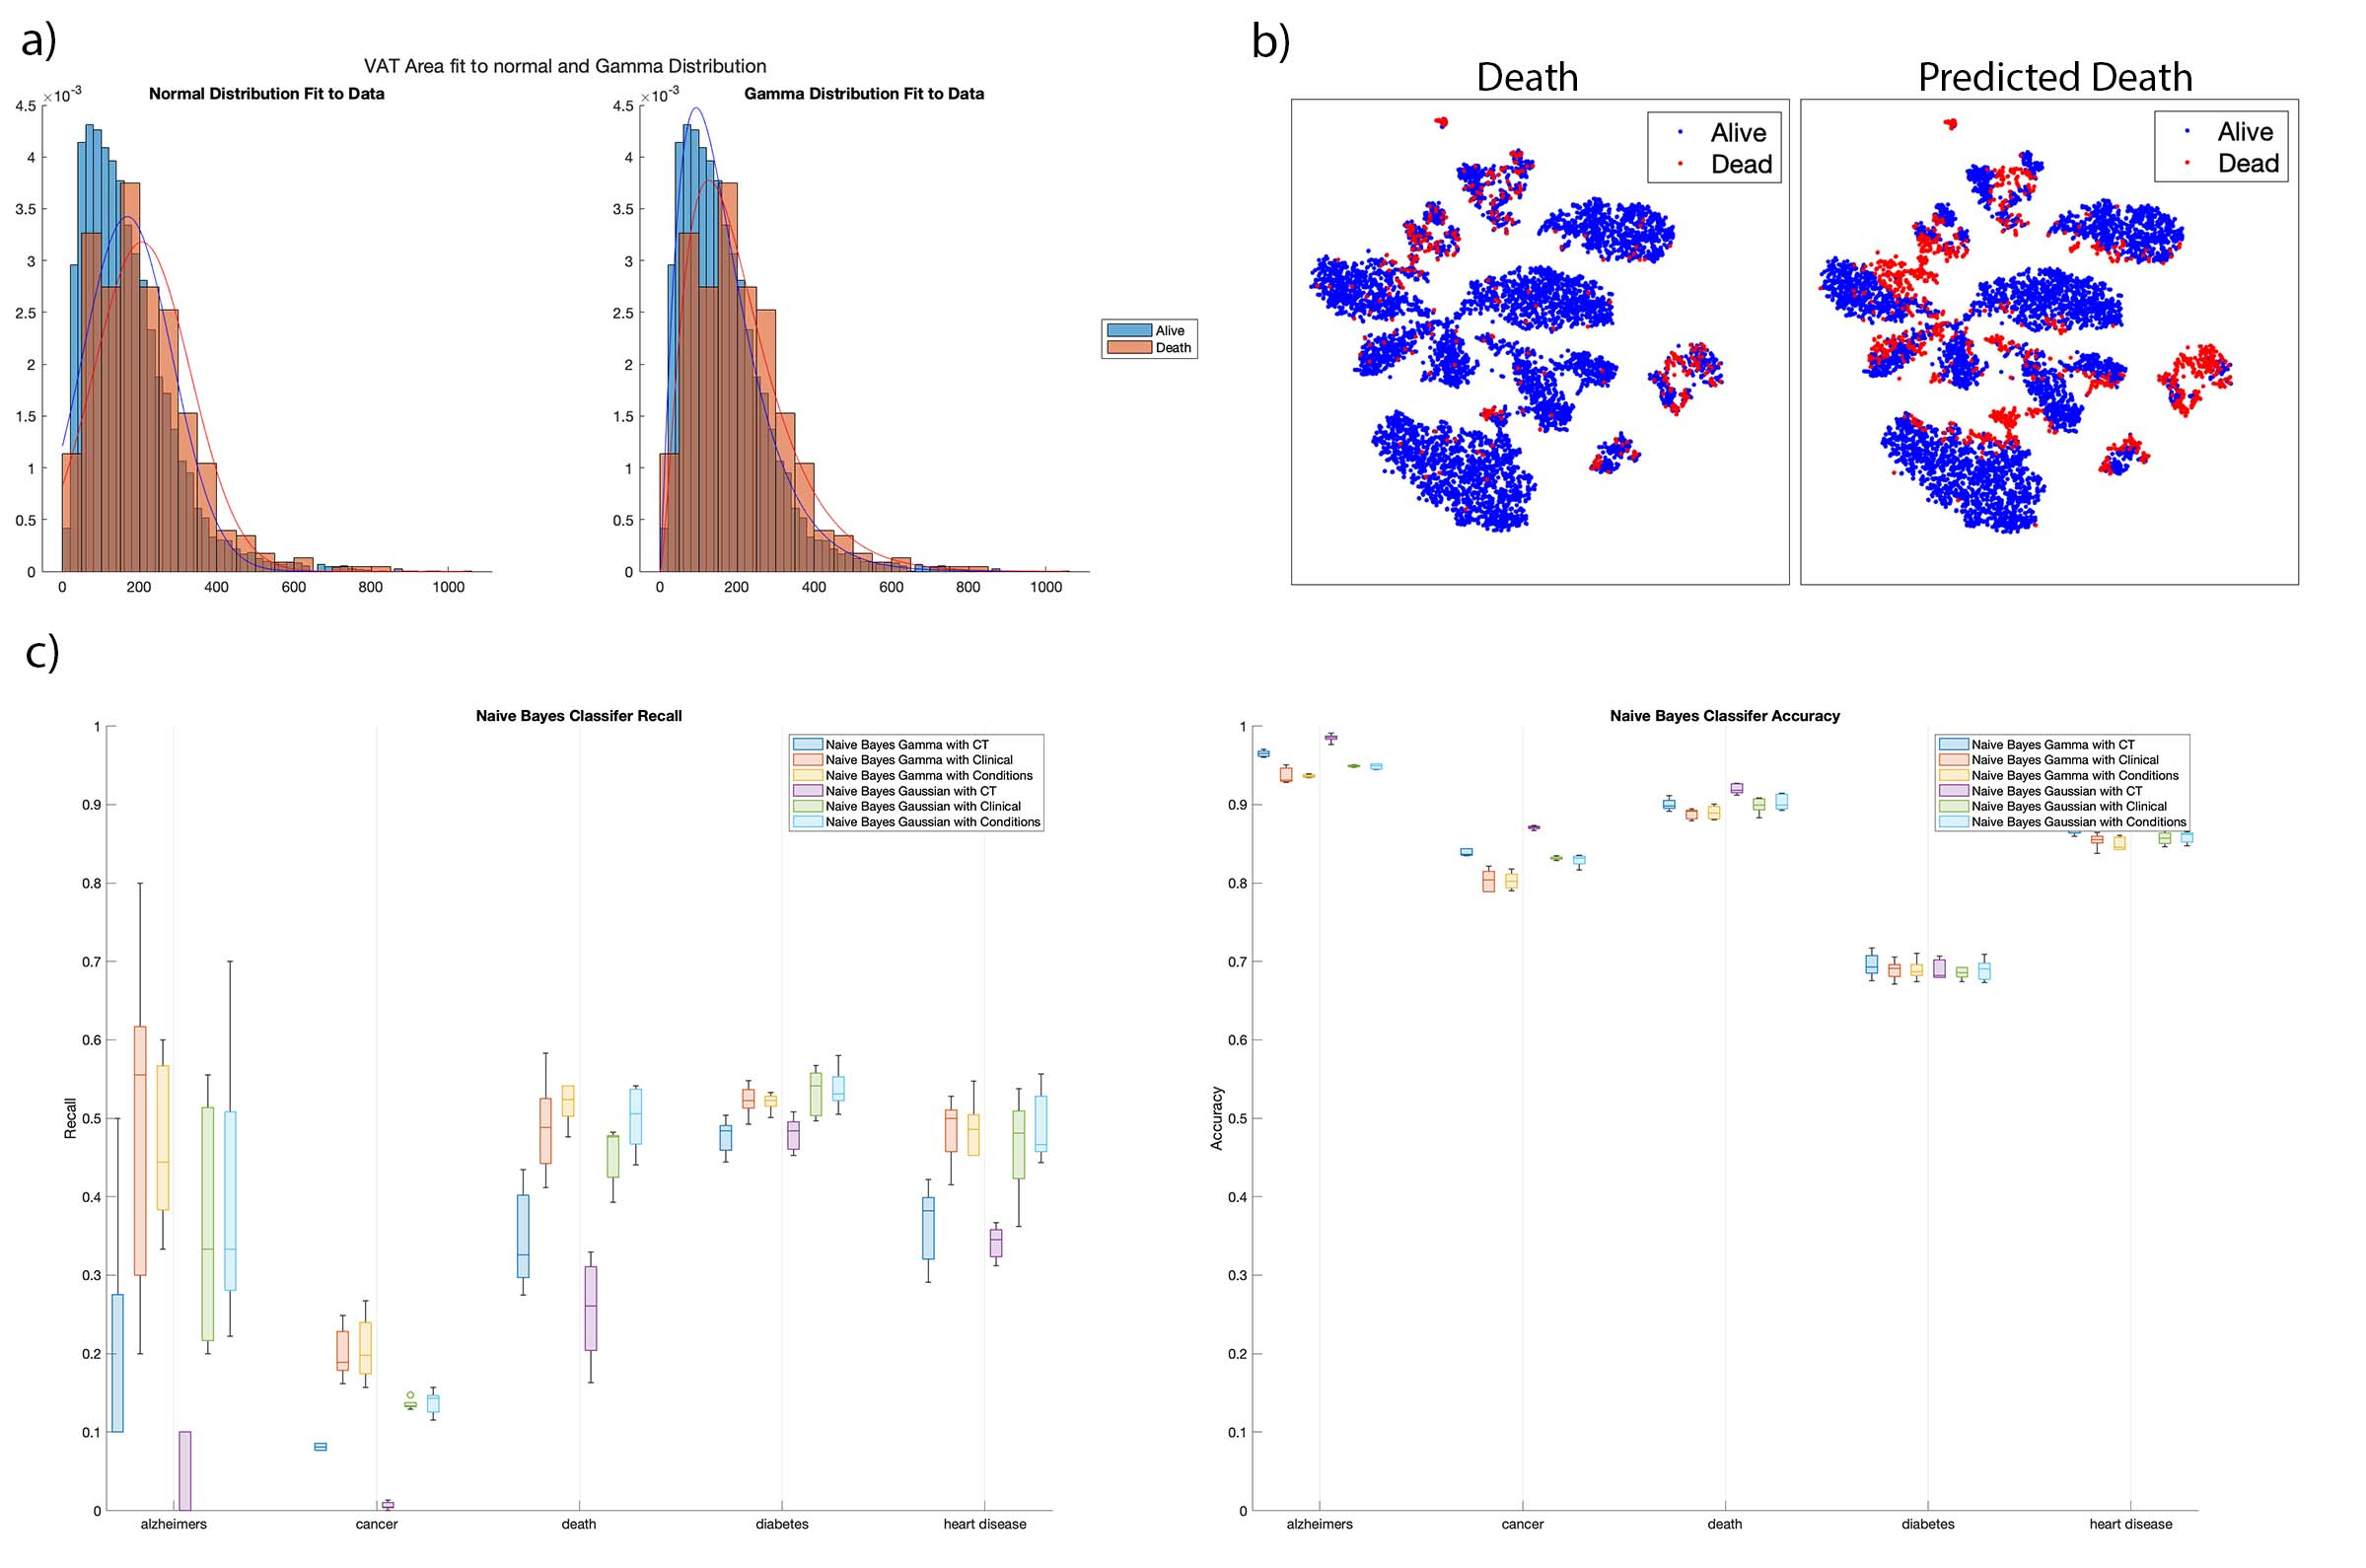
\includegraphics[width=.95 \textwidth]{results/figure_1.jpg}
\caption{Naive Bayes classifier results. a) Histograms of the VAT area feature are show. The solid lines indicate the distribution inferred by the Bayes Classifier. In the left plot, the estimated distribution of alive and dead patients using a normal distribution is very similar. The right plot demonstrates that the learned Gamma distributions better fit the data. b)  t-SNE projections of the CT with clinical data and conditions is shown. Patients are colored by their survival or predicted survival using a naive bayes classifier with gamma distributions.  Patients predicted to have died (red) are localized in regions in which many patients actually die, indicating the classifier is correctly identify at risk patients are shown for the CT with clinical data and condition indicators dataset. c) The classification recall and accuracy for predicting the clinical conditions of Alzheimer's, cancer, death,  diabetes, and heart disease for all three datasets. The models perform optimally when trained with the gamma distributions and when the clinical data is used in combination with CT.  Performance is only slightly enhanced when the additional condition indicators are added.}
\end{figure} 

In general, the naive Bayes classifier performs well. Figure 1.b demonstrates prediction made on the CT with clinical and condition indicator dataset. Individuals for which death is predicted are in similar locations to people who actually died. This suggests that the classifier is correctly identify important features for predicting overall health of the individual. Although the t-SNE plot is suggest of an accurate model, the recall of the naive Bayes classifier is relatively low without the addition of CT data. This hold true for all clinical conditions except for diabetes for which the recall is approximately the same on all three datasets. When clinical data is added the recall of the model always improves. The greatest improvements are in predicting death, which indicates factors such as age, tobacco use, alcohol abuse, and computed health metrics, improve the prediction of overall health when coupled with CT data. 

\begin{figure}[ht!]
\centering
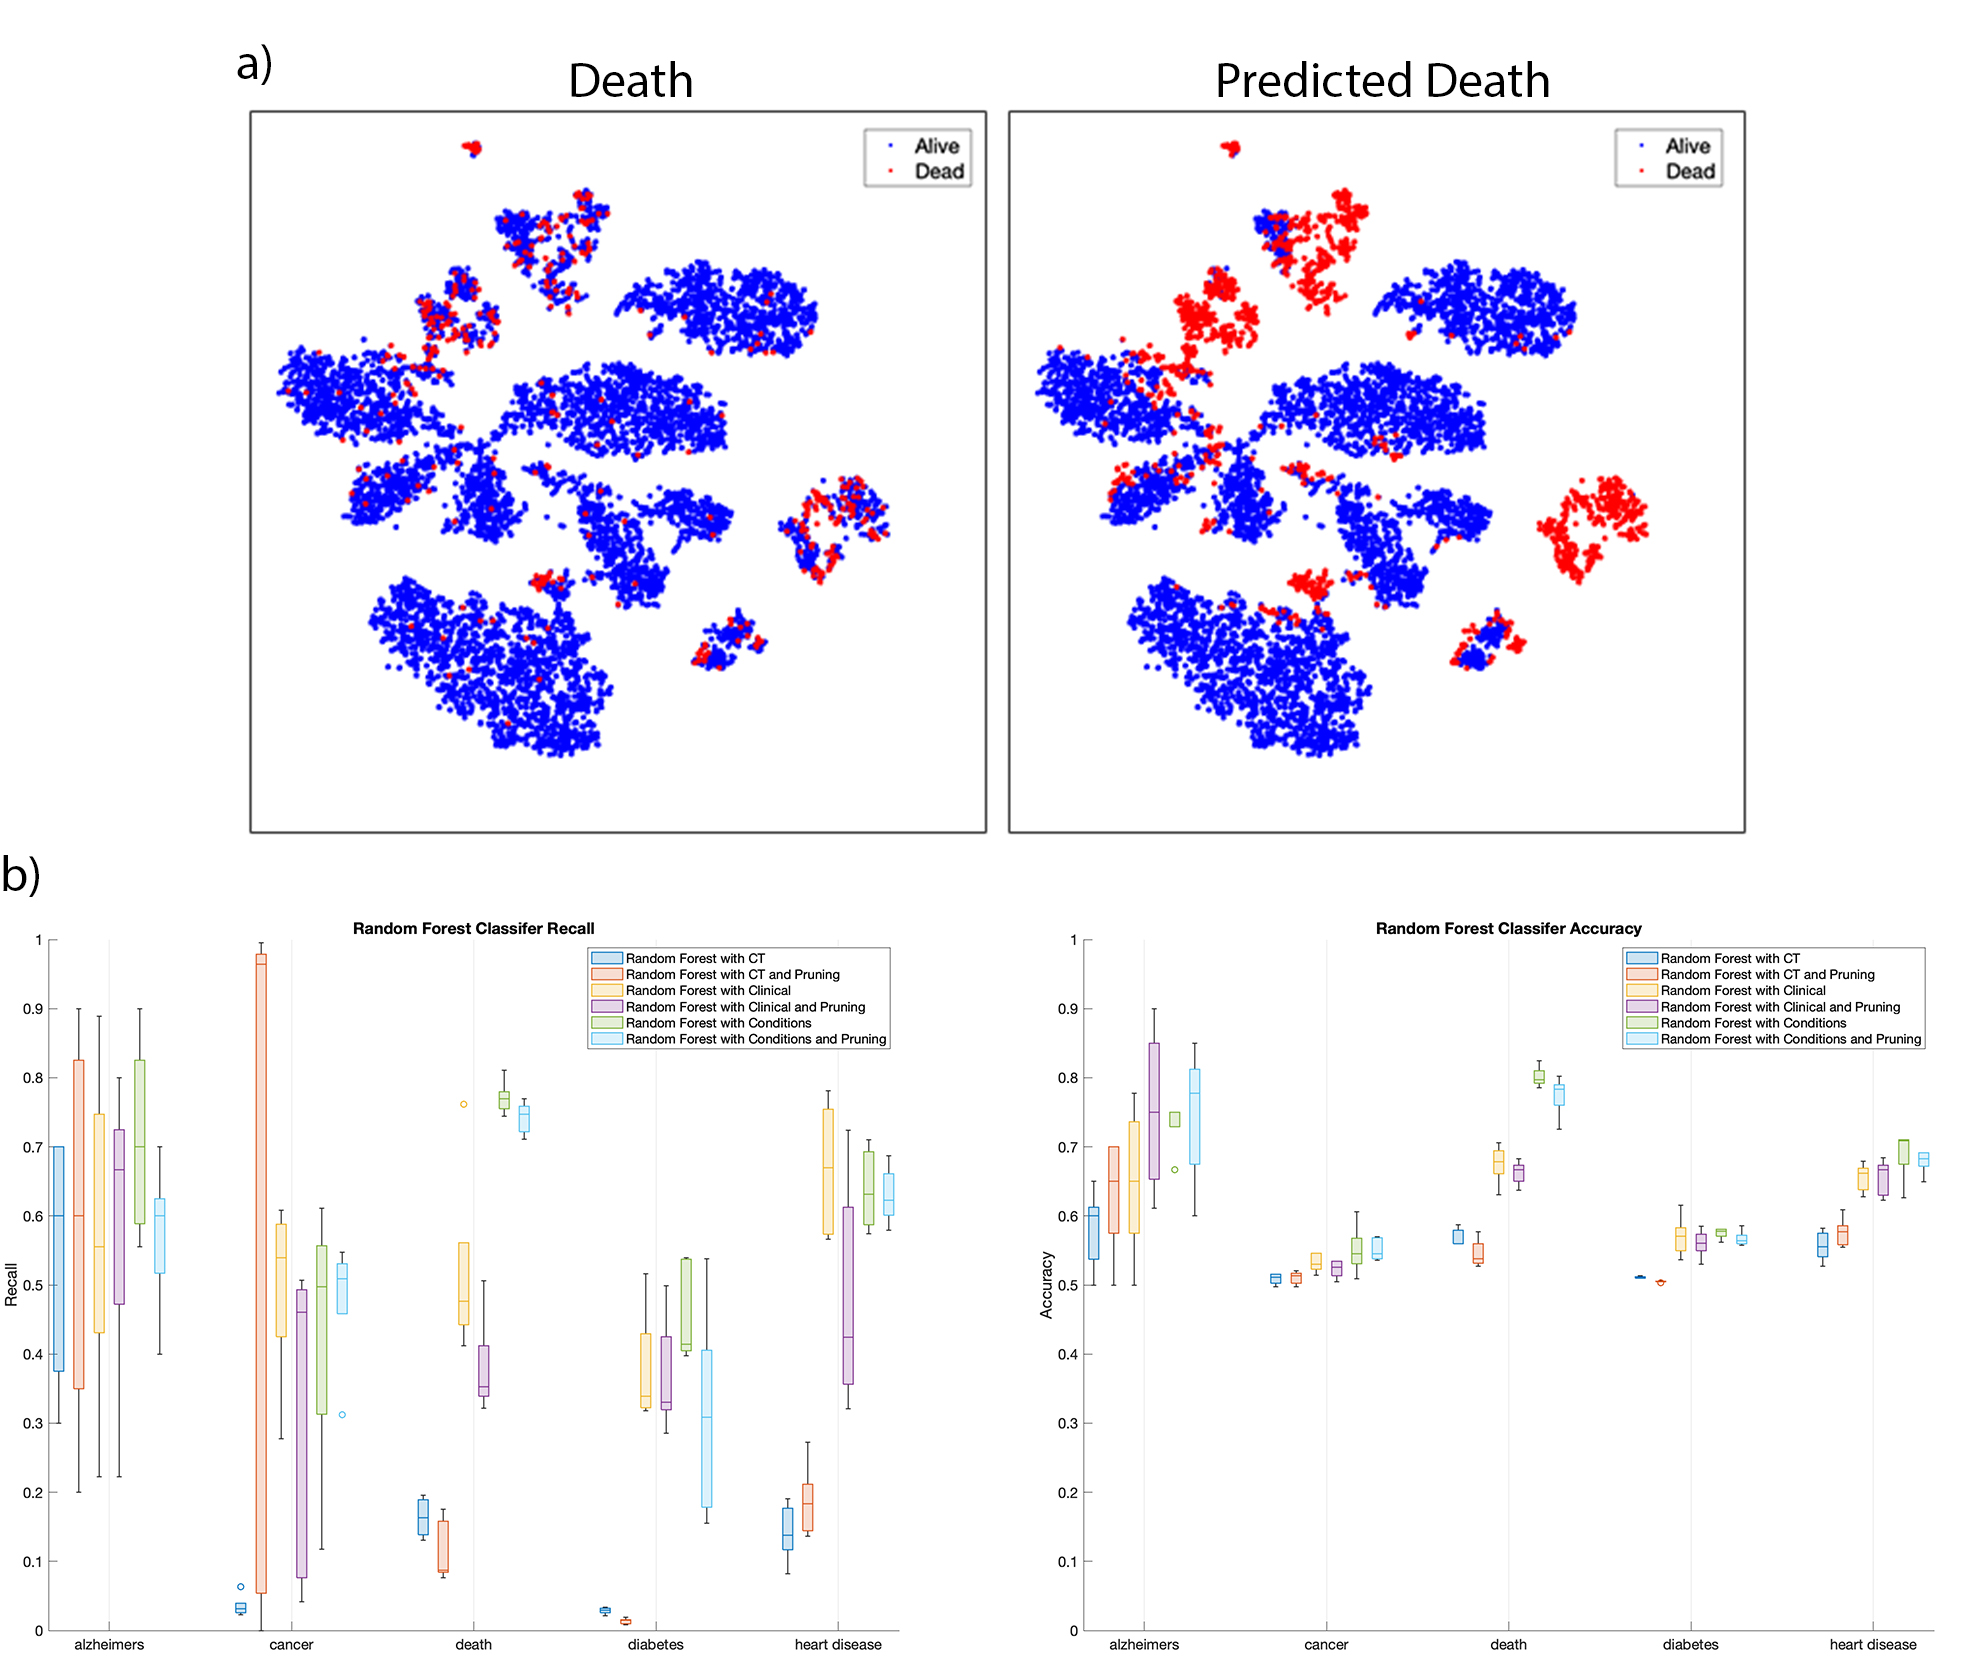
\includegraphics[width=.98\textwidth]{results/figure_2.jpg}
\caption{Random Forest classifier results. a) t-SNE projections of the CT with clinical data and conditions is shown. Patients are colored by their survival or predicted survival using random forest regression  Patients predicted to have died (red) are localized in regions in which many patients actually die, indicating the classifier is correctly identify at risk patients are shown for the CT with clinical data and condition indicators dataset. The regions or predicted death are more closely associated with actual regions of predicted death than with the Bayes classifier. c) The classification recall and accuracy for predicting the clinical conditions of Alzheimer's, cancer, death, diabetes, and heart disease for all three datasets. The random forest model drastically improves with the addition of clinical data and condition indicators. For comparison, a random forest model without pruning and pruning is shown. Pruning decreases both recall and accuracy.}
\end{figure} 

In comparison to the naive Bayes classifier, the random forest classifier performs even more poorly on CT data alone, as demonstrated in Figure 2.b. In this case the model achieved a recall of only around 15 percent and an overall classification accuracy of 50 percents. However, with the addition of clinical data and condition indicators, the recall and accuracy improve significantly. When predicting death, a recall of 80 percent is obtained and the overall classification accuracy improves to 80 percent as well. This indicates that that labeled conditions are more predictive than CT alone. The t-SNE in figure 2.a, we can see that the random forest model  correctly identifies locations of the t-SNE enriched for actual death. This suggests that the model is correctly able to identify important factors for predicting death and that these factors can be used to identify individuals who are at risk of adverse health. When comparing the t-SNE in Figure 2.a to Figure 1.b, it is clear that the Random Forest model is more selective than the Bayes classifier. Specifically, there are fewer regions of the t-SNE that are labeled as high risk of death in the random forest model are much smaller and more specific than the Bayes classifier. 

\begin{figure}[!h]
\centering
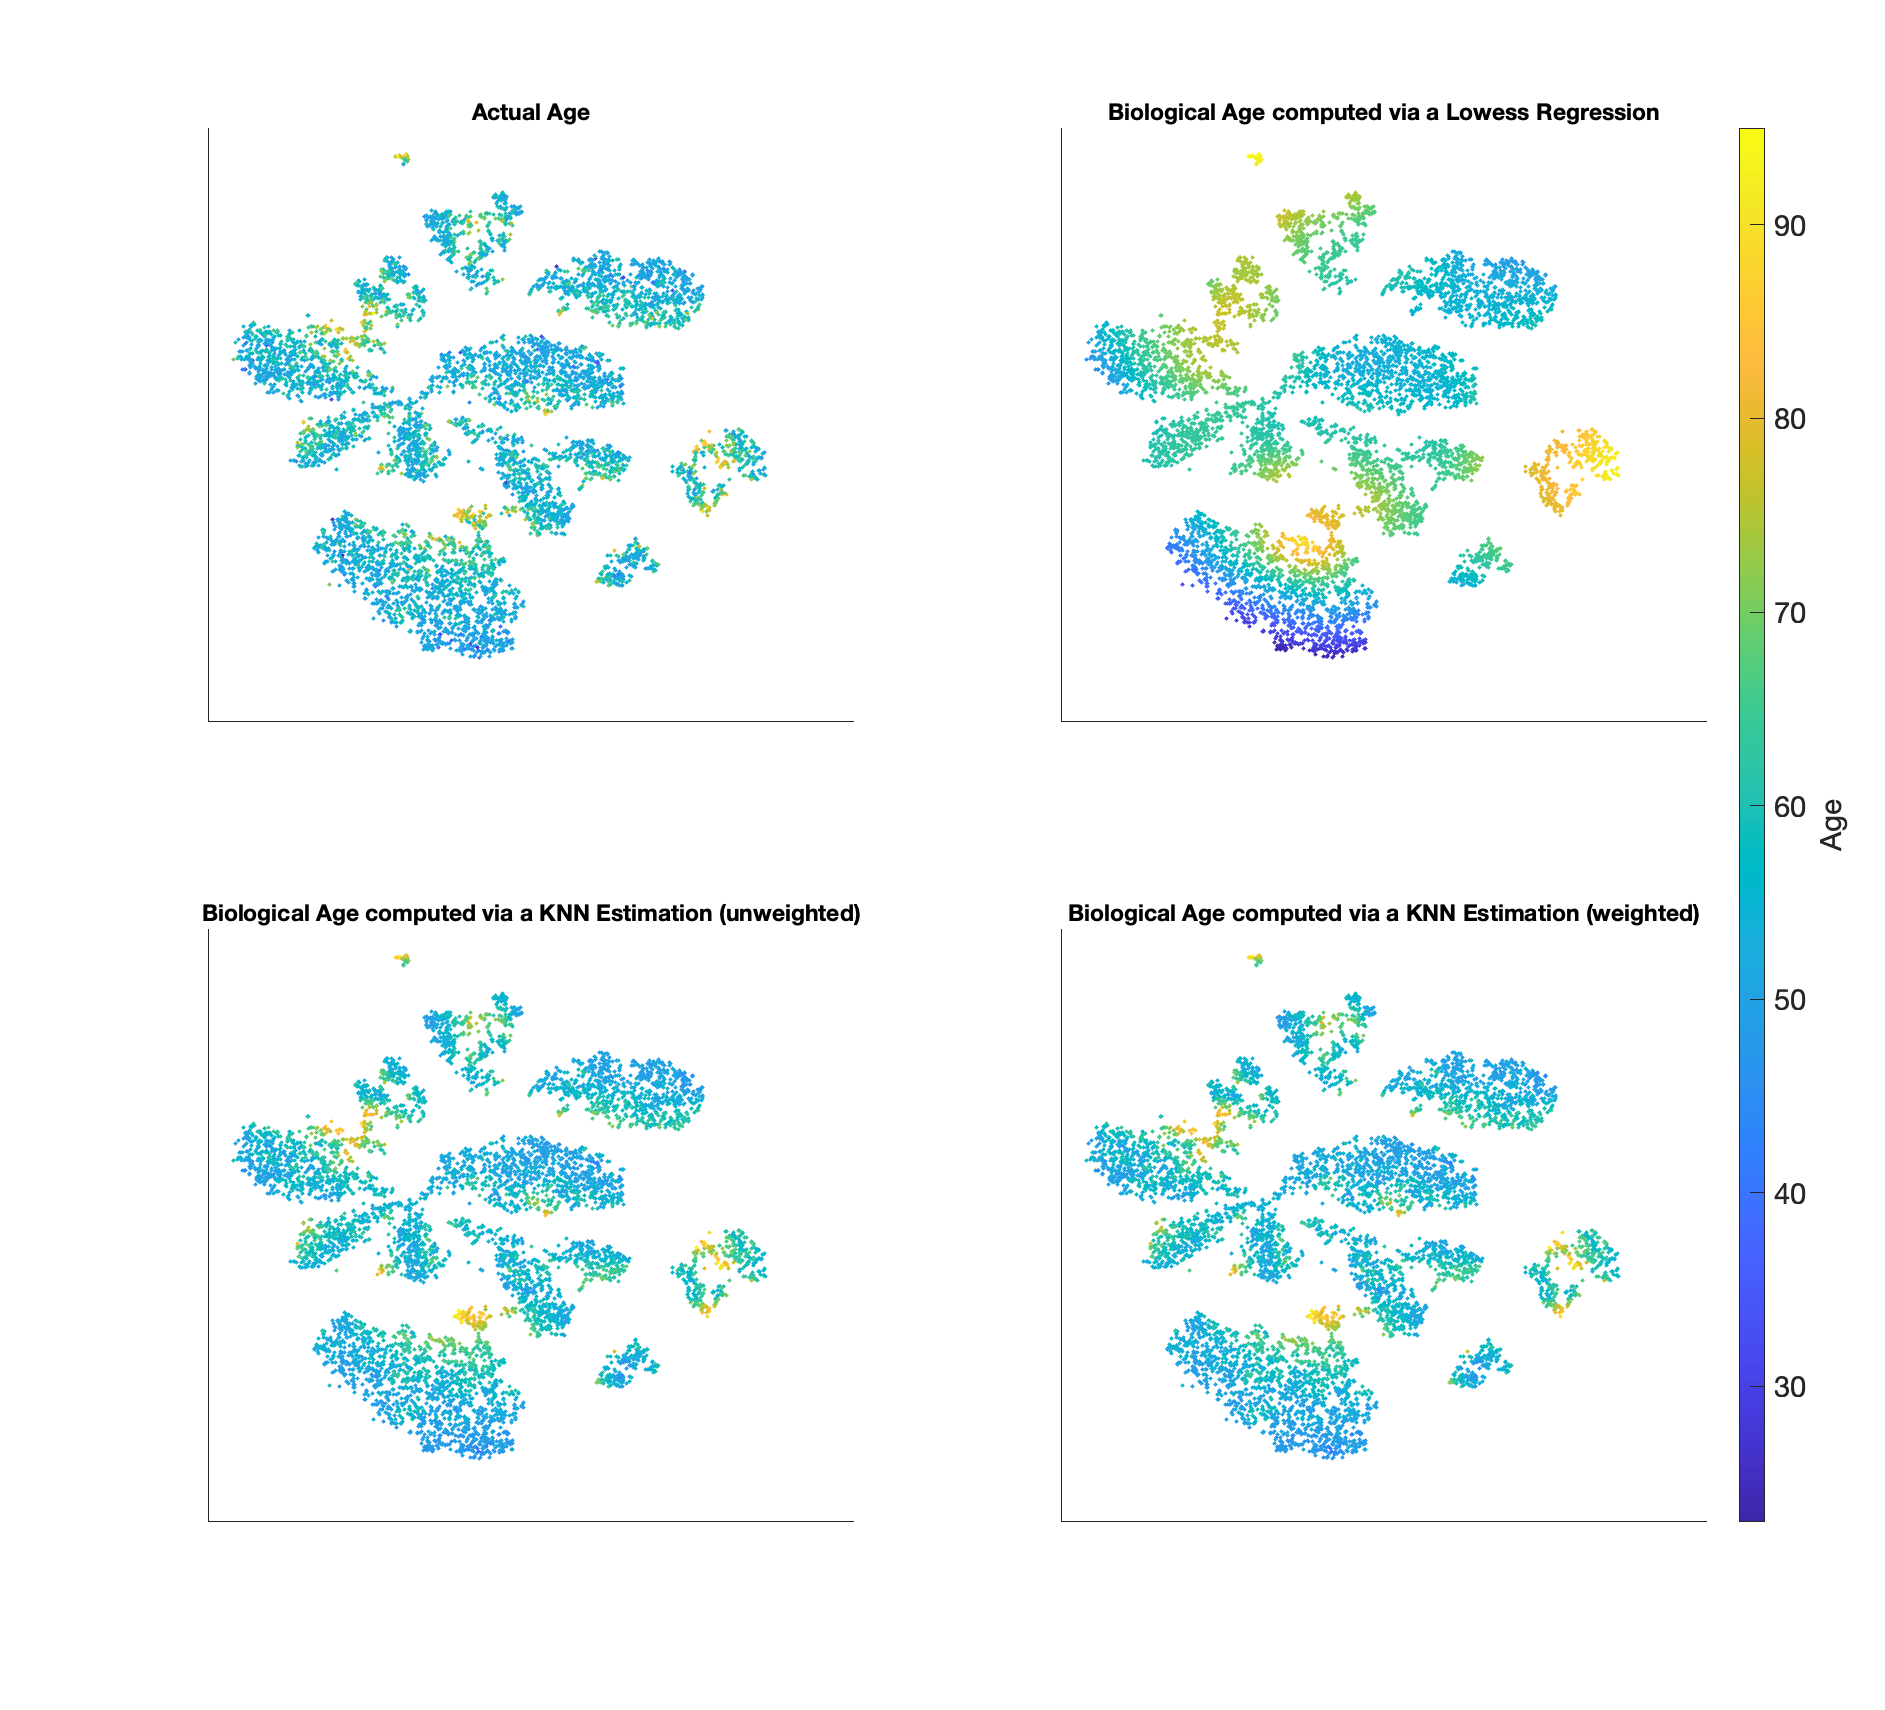
\includegraphics[width=.9\textwidth]{results/Conditions_data_bio_age.png}
\caption{Age and Biological Age Predictions. The top left plot shows actual ages, Regions of the t-SNE related to death have slightly elevated ages. The LOWESS method increase the contrast between regions and ages. The regions of t-SNE related to death have much higher ages than the corresponding actual ages. Both KNN methods (unweighted and weighted) show elevation in ages in areas associated with death but to a far lesser extent than the LOWESS. }
\end{figure}
 
In addition to comparing the Random forest metrics to the Bayes model, we wanted to study the affect of pruning on the accuracy of the random forest model. Typically pruning is used to capture complex interactions between variables by growing a large tree. Then, unnecessary branches are removed by comparing to a test holdout. When we applied pruning to trees in our random forest, we see a decrease in performance. This result is unexpected since pruning methods have been used to improve performance of trees \cite{nortonGeneratingBetterDecision1989}, specifically when data is complex and highly related. We hypothesis that the decrease in performance may be a result of the size of the dataset. Specifically, our holdout dataset for pruning is relatively small and may not contain enough variability to fully capture the complexity of the data. This may result in over-pruning as only a few branches may be needed to predict the small holdout dataset. 

Finally, we attempted to build models to predict a meaningful biological age from CT with clinical and condition indicators data. To accomplish this task, we wanted to use the features of the dataset, and train on age to get a meaningful estimate of overall health. We attempted to to do this with two different strategies, LOWESS regression on t-SNE embedding coordinates, and KNN regression on normalized features. Figure 3 demonstrates the relationship between actual age and the predicted biological age using the three different methods. All three biological age computation methods increase the contrast of between regions with young and old individuals when compared to actual age. When we compare this with the death t-SNE in Figure 1.b, we see that the regions enriched for older individuals corresponds with increased death. This is especially true for the LOWESS computed ages which drastically increase in regions associated with death. This indicates that increase in our biological age metric is suggestive of risk of death as desired. 


\section{Conclusions and Future Work}
Our results indicate that both a naive Bayes and random forest classifier are valid methods for constructing a risk prediction model based on CT data and clinical data. The naive Bayes model performs better on CT data alone and the random forest model performs well when integrated with clinical data. Both models produce predictions that are consistent with actual adverse health effects, and in particular predict the risk of death well. We have also developed methods for computing a biologically meaningful age using LOWESS regression and KNN neighbors. Both methods produce biological ages consistent with actual ages, but increase biological ages in t-SNE regions enriched with death. In particular, LOWESS regression on t-SNE embedded data produces larger amounts of contrast between regions and thus may be better indicator of overall health. 

In the future, we would like to extend the naive Bayes model to a graphical Bayesian model. Many of the variables that we have considered in our CT experiment are likely to exhibit dependency relationships which violates the independence assumption of the naive Bayes model. We can account for this by allowing limited dependency by constructing a bayesian network and thus can improve are results. Bayesian networks also provide context of which variables most directly effect the given condition and thus can be incredibly valuable for determining risk factors. We would also like to improve our random forest model. Our current implementation is limiting on the maximum number of trees that can be used. This is mostly because our tree traversal algorithm is relatively slow. If we improve this part of our model, we could increase performance by allowing more tree in our forest. Finally, we would like to benchmark are biological age with actual age. We could build a simple model to try and predict death from biological age and actual age alone. If the biological age is as predictive death as the t-SNE suggests we would expect a higher accuracy of prediction given the biological age feature.  


\section{References}
Code used to produce the results presented in this paper is located here, . 

\bibliographystyle{abbrv} 
\bibliography{CS_Final_report}




\end{document} 
































